\chapter{Асимметрия и эксцесс нормального распределния}
\label{ch:chap4}

\section*{Асимметрия и эксцесс распределения}

\subsection*{1. Асимметрия (Skewness)}

Асимметрия показывает, насколько распределение \emph{скошено} относительно своего среднего:

\begin{itemize}
    \item Если $\text{Skewness} = 0$, распределение симметрично (как нормальное).
    \item Если $\text{Skewness} > 0$, хвост распределения длиннее вправо (распределение скошено вправо).
    \item Если $\text{Skewness} < 0$, хвост распределения длиннее влево (распределение скошено влево).
\end{itemize}

Для нормального распределения:

\[
\text{Skewness} = 0
\]

То есть нормальное распределение симметрично относительно среднего.

\subsection*{2. Эксцесс (Kurtosis)}

Эксцесс характеризует \emph{островерхость} распределения — насколько высокая или плоская вершина у графика плотности:

\begin{itemize}
    \item Для нормального распределения $\text{Kurtosis} = 3$.
    \item Часто используют избыточный эксцесс (Excess Kurtosis):
    \[
    \text{Excess Kurtosis} = \text{Kurtosis} - 3
    \]
    чтобы нормальное распределение имело избыточный эксцесс $0$.
\end{itemize}

Интерпретация избыточного эксцесса:

\begin{itemize}
    \item $\text{Excess Kurtosis} = 0$ $\rightarrow$ нормальное распределение (стандартная «колоколообразная» форма).
    \item $\text{Excess Kurtosis} > 0$ $\rightarrow$ пики выше и хвосты тяжелее (лепестковая форма).
    \item $\text{Excess Kurtosis} < 0$ $\rightarrow$ более плоская вершина и тонкие хвосты (плосковершинная форма).
\end{itemize}

Реализация:

\begin{figure}[H]
    \centering
    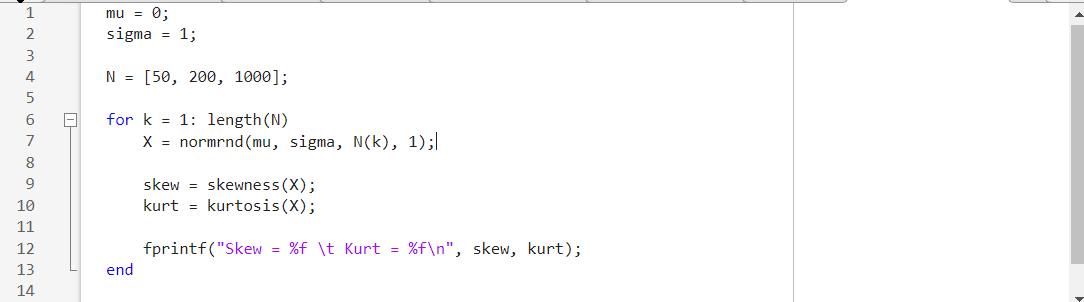
\includegraphics[width=1.0\textwidth]{skew&kurt.png}
    \caption{Пример вычисления асимметрии и эксцесса для нормального стандартного распределения}
\end{figure}


\endinput